\section{Early stage researchers}
\label{esrs}
12 ESRs form the core of the network, with the training and partnerships providing a scaffold for the completion of their respective outcomes. Each ESR is enrolled as a doctoral student at a partner university for 3 years, during which they complete secondments in HEP and industry, as illustrated in Figure~\ref{esr-diagram}. The university of enrolment is generally also the hosting institution, where the majority of the doctoral study is completed (industry-centred ESR positions are enrolled at a university near to the respective industry partner). A secondment in HEP is undertaken either at another partner university or a partner research institute. Each ESR (with the exception of those in industry-centred positions) also undertakes a secondment in industry, working on an RTA project relevant to their research with an industry partner.

\begin{figure*}[h!]
    \centering
    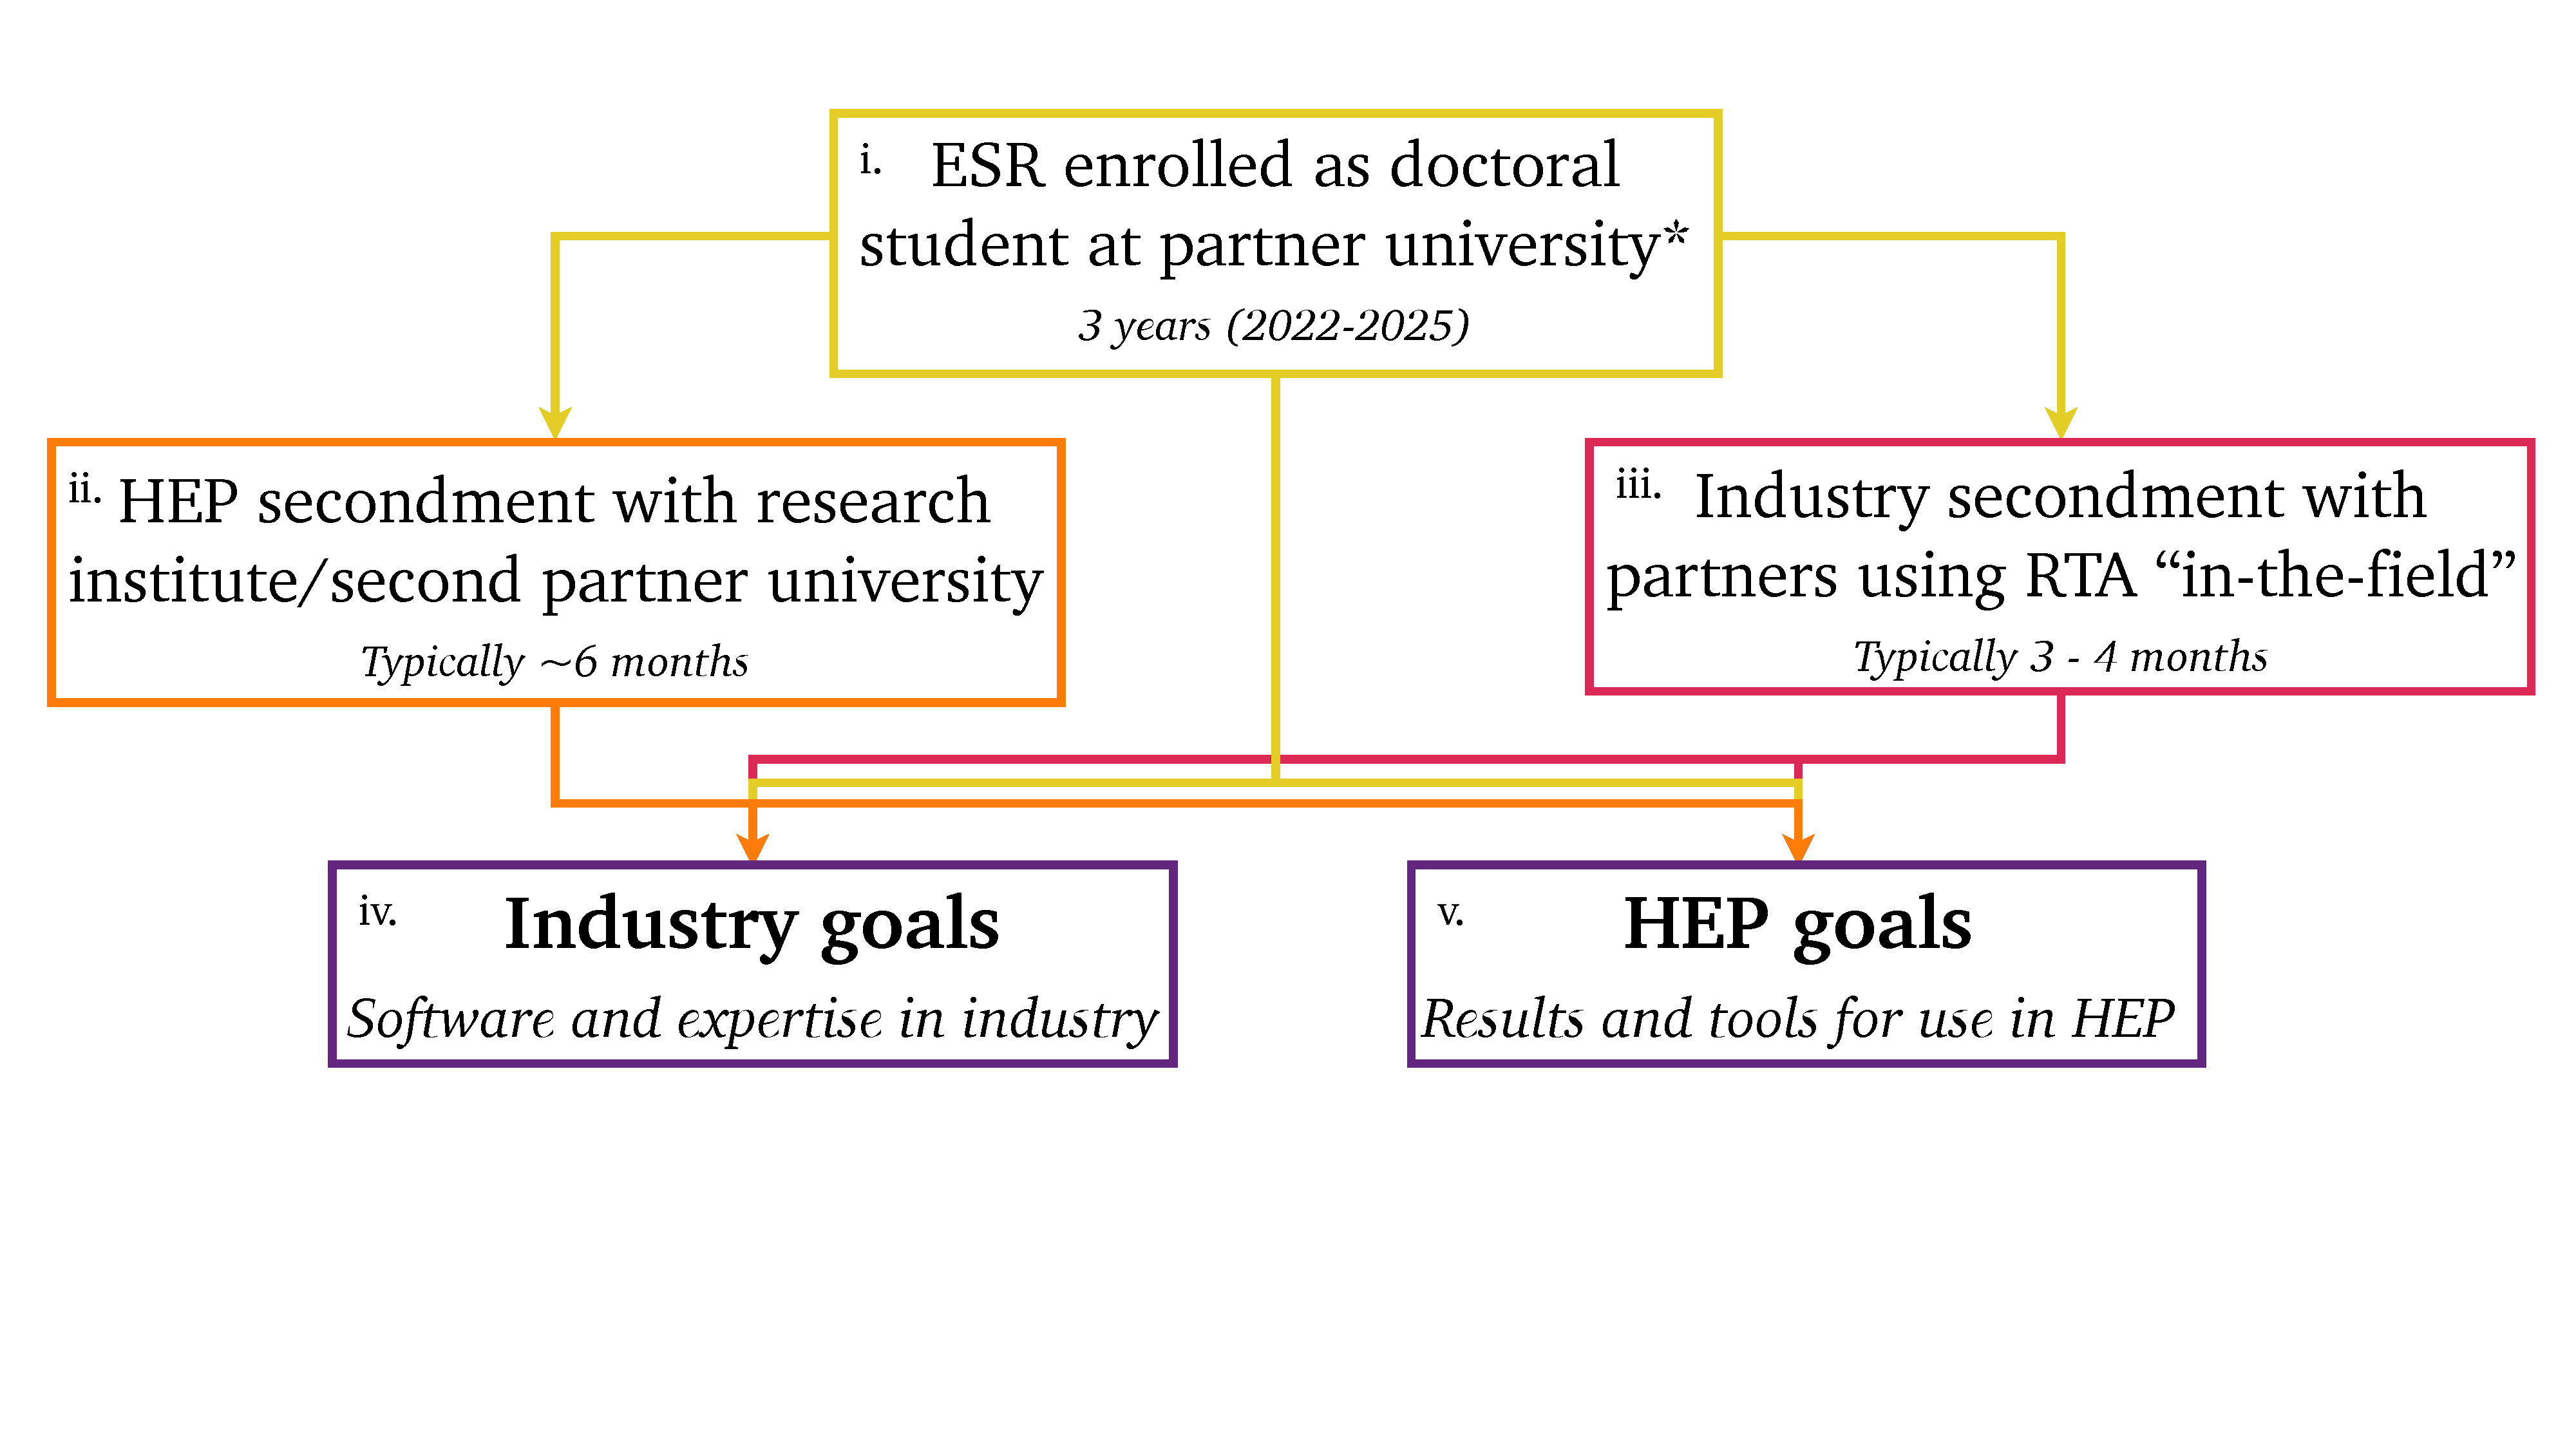
\includegraphics[width=\linewidth,clip]{/Users/jgooding/Documents/SMARTHEP/CHEP2023/CHEP2023/proceedings/figures/esr-diagram.pdf}
    \caption{Structure of a SMARTHEP ESR position. Each ESR is enrolled (i.), during which they will undertake secondments with network partners in HEP (ii.) and industry (iii.). Through the combination of primary and secondment work, each ESR will complete goals in HEP (iv.) and industry (v.), discussed in further detail in Section~\ref{goals}. Precise durations of the secondments vary between ESR positions.}
    \label{esr-diagram}
\end{figure*}

To illustrate further the structure of a SMARTHEP ESR position 4 examples are given:
\begin{itemize}
    \item  Laura Boggia, one of two industry-centred ESRs, is researching fraud detection using real-time rule induction at Sorbonne University, working with industry partner IBM. A secondment with the CNRS research institute is planned, in which similar techniques will be applied to the classification of HEP observations.
    \item Jamie Gooding, based at Technische Universit\"at Dortmund, is investigating the real-time selection of dilepton $B_{(s)}^0$ decays at LHCb. Time spent working at CERN will contribute to the commissioning of the Run 3 LHCb trigger. A secondment developing real-time traffic data processing techniques at Ximantis will promote a synergy in ML applications between industry and HEP.
    \item Carlos Cocha is based at the University of Heidelberg, working on real-time searches for Dark Photons at LHCb, furthered by collaboration with the University of Milano-Bicocca. An industry secondment with Verizon Connect is planned, applying ML expertise to the real-time processing of vehicle data.
    \item Joachim Hansen is developing the real-time calibration of the ALICE Time Projection Chamber, working at Lund University. This commissioning work will be supported by a secondment at CERN. An additional secondment will also take place with Ximantis to further develop skills in ML applications.
\end{itemize}